\documentclass{article}

\usepackage[version=3]{mhchem} % Package for chemical equation typesetting
\usepackage{siunitx} % Provides the \SI{}{} and \si{} command for typesetting SI units
\usepackage{natbib} % Required to change bibliography style to APA
\usepackage{graphicx}
\usepackage{mathtools}
\usepackage{amssymb}
\usepackage{amsthm}
\usepackage[italian]{babel}
\usepackage{stackengine}
\usepackage{graphicx,ifthen}
\usepackage{amsmath}
\usepackage{hyperref}
\usepackage{upgreek}
\usepackage{bm}

\renewcommand{\labelenumi}{\alph{enumi}.} % Make numbering in the enumerate environment by letter rather than number (e.g. section 6)

\title{Esperienza III: \\ spettroscopio}
\author{Manuel G. Moretti\footnote{email: manuel.moretti560@edu.unito.it}}
\date{Luglio 2024}

\begin{document}

\maketitle

\begin{center}
\begin{tabular}{l r}
Esperimentazioni II corso B & A.A. 2023/24 \\
Modulo II & Universit\'{a} degli Studi di Torino \\
\end{tabular}
\end{center}

\begin{abstract}
In questa esperienza tramite l'utilizzo di uno spettroscopio di Kirchhoff-Bunsen e di un reticolo di diffrazione si è stimata la lunghezza d'onda delle onde elettromagnetiche componenti lo spettro di emissione del mercurio. Sostituendo in seguito il reticolo di diffrazione con un prisma di vetro crown si è ricavato l'andamento dell'indice di rifrazione di quest'ultimo in funzione della lunghezza d'onda.
\end{abstract}

\section{Obiettivi della misura}
Gli obiettivi di questa esperienza sono di misurare la lunghezza d'onda delle righe presenti nello spettro di emissione del mercurio e di ricavare l'andamento dell'indice di rifrazione di un prisma di vetro in funzione della lunghezza d'onda.

\section{Configurazione dell'apparato sperimentale}
L'apparato sperimentale di compone di uno spettroscopio di Kirchhoff-Bunsen e di una lampada ai vapori di mercurio. 

Lo spettroscopio è composto dalle seguenti parti: un cannocchiale oculare, attraverso il quale è possibile vedere le righe di emissione; un collimatore, che permette di incanalare i raggi luminosi generati dalla sorgente; una piattaforma girevole dotata di un goniometro con nonio. Il cannocchiale può essere inoltre ruotato per misurare l'angolazione delle righe spettrali tramite il nonio ad esso solidale.

Sulla piattaforma girevole vengono posti prima un reticolo di diffrazione, consistente in una sottile lastra su cui è incisa una trama di sottili linee parallele a distanze confrontabili con la lunghezza d'onda della luce, e poi un prisma di vetro crown.

\section{Raccolta ed elaborazione dei dati}
\subsection{Stima delle lunghezze d'onda tramite un reticolo di diffrazione}
La raccolta dei dati per questa parte di esperienza è consistita in una serie di misure dell'angolazione a cui si presentavano le righe spettrali. Tramite il cannocchiale oculare infatti, partendo dalla riga centrale, si è misurata l'angolazione delle righe del primo, secondo e terzo ordine. In particolare, si sono osservate le righe di colore viola, verde scuro, verde chiaro, giallo e rosso. Le misure degli angoli sono state effettuate con il goniometro con una precisione di un grado, insieme il nonio con una precisione di un primo. 

Per ogni riga di ogni ordine si è quindi stimata la corrispondente lunghezza d'onda tramite la formula
\begin{equation}
    \label{eq:lambda reticolo}
    m\lambda=p\sin{\theta},
\end{equation}
dove $m$ indica l'ordine corrispondente alla riga, $\theta$ indica l'angolo misurato e $p$ corrisponde al passo del reticolo, in questo caso il passo è di $p=300$ linee/mm.

Dunque, dopo aver effettuato tre misure dell'angolazione di ogni riga per ogni ordine, si è effettuata una media tra le misure di ogni riga la cui incertezza corrisponde alla semidispersione tra le tre misure. Successivamente, si è effettuato un test di Gauss tra le medie di ogni riga con quelle degli altri ordini per verificare la compatibilità di esse. Quindi, si è calcolata la media delle medie di ogni riga, ottenendo pertanto una stima della lunghezza d'onda di ogni riga. I risultati finali di questo processo sono raccolti nella seguente tabella.
\begin{table}[ht]
    \centering
    \begin{tabular}{|c|c|}
        \hline
        \textbf{Riga} & \textbf{Lunghezza d'onda [nm]} \\
        \hline
        Viola & $405.31\pm0.37$ \\
        \hline
        Blu & $435.22\pm0.37$ \\
        \hline
        Verde scuro & $491.91\pm0.36$ \\
        \hline
        Verde chiaro & $545.40\pm0.20$ \\
        \hline
        Giallo & $578.70\pm0.24$ \\
        \hline
        Rosso & $621.54\pm0.35$ \\
        \hline
    \end{tabular}
    \caption{stima lunghezza d'onda di ogni riga}
    \label{tab:stima lunghezza d'onda}
\end{table}

\subsection{Stima dell'indice di rifrazione di un prisma}
La raccolta dei dati della secondo parte è essenzialmente analoga rispetto a quanto detto con il reticolo di diffrazione. L'unica differenza consiste nel soddisfare la condizione di deviazione minima. Essa corrisponde a posizionare il prisma ad un'angolazione tale che le righe dello spettro deviato da esso sono il più vicine possibile alla direzione del fascio incidente. In altre parole, l'angolo di minima deviazione corrisponde a quando l'angolo di incidenza è uguale all'angolo di emersione.
\begin{figure}[ht]
    \centering
    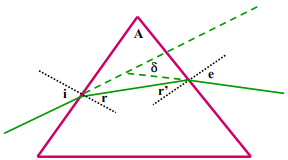
\includegraphics[width=0.5\linewidth]{Immagini/angoloD.png}
    \caption{cammino del raggio all'interno del prisma}
    \label{fig:cammino ottico prisma}
\end{figure}

In questa condizione risulta che $A=2r$, come si vede in figura \ref{fig:cammino ottico prisma}, e si può ricavare la relazione
\begin{equation}
    \label{eq:n prisma}
    n=\frac{\sin{\frac{\delta_{min}+A}{2}}}{\sin{\frac{A}{2}}},
\end{equation}
dove $\delta_{min}$ corrisponde per l'appunto all'angolo di minima deviazione del prisma. Operativamente per trovare l'angolo di minima deviazione prima di tutto si misura l'angolazione della riga corrisponde alla fenditura, poi si riposiziona il prisma sulla piattaforma e tramite il cannocchiale si seguono le righe spettrali fino al punto in cui esse non "invertono il moto", l'angolo a cui ciò avviene è proprio l'angolo di minima deviazione.

I dati ottenuti in questa parte di esperienza sono raccolti nella seguente tabella.
\begin{table}[h]
    \centering
    \begin{tabular}{|c|c|}
        \hline
        \textbf{Riga} & \textbf{\bm{$\delta_{min}$} [rad]} \\
        \hline
        Rosso & $0.79\pm0.03$ \\
        \hline
        Giallo & $0.80\pm0.03$ \\
        \hline
        Verde chiaro & $0.80\pm0.03$ \\
        \hline
        Verde scuro & $0.82\pm0.03$ \\
        \hline
        Blu & $0.84\pm0.03$ \\
        \hline
        Viola & $0.85\pm0.03$ \\
        \hline
    \end{tabular}
    \caption{angolo di minima deviazione di ogni riga}
    \label{tab:angolo minima deviazione}
\end{table}
\newpage
\section{Risultati e conclusioni}
I dati raccolti nella tabella \ref{tab:stima lunghezza d'onda} devono essere ora confrontati con le misure effettuate con lo spettrofotometro. Queste ultime sono raccolte nella seguente tabella.
\begin{table}[ht]
    \centering
    \begin{tabular}{|c|c|}
        \hline
        \textbf{Riga} & \textbf{Lunghezza d'onda [nm]} \\
        \hline
        Viola & $405.02\pm0.60$ \\
        \hline
        Blu & $436.02\pm0.60$ \\
        \hline
        Verde scuro & $491.52\pm0.21$ \\
        \hline
        Verde chiaro & $546.02\pm1.20$ \\
        \hline
        Giallo & $578.02\pm1.27$ \\
        \hline
        Rosso & $620.02\pm1.06$ \\
        \hline
    \end{tabular}
    \caption{misure lunghezza d'onda con spettrofotometro}
    \label{tab:misure spettrofotometro}
\end{table}

Effettuando dunque un test di Gauss tra le misure della lunghezza d'onda delle righe dello stesso colore si ottengono i seguenti valori di $Z$.
\begin{table}[ht]
    \centering
    \begin{tabular}{|c|c|}
        \hline
        \textbf{Riga} & \textbf{Valore di Z} \\
        \hline
        Viola & $0.44$ \\
        \hline
        Blu & $1.11$ \\
        \hline
        Verde scuro & $0.94$ \\
        \hline
        Verde chiaro & $0.49$ \\
        \hline
        Giallo & $0.53$ \\
        \hline
        Rosso & $1.38$ \\
        \hline
    \end{tabular}
    \caption{test di Gauss tra righe dello stesso colore}
    \label{tab:test di gauss lunghezze d'onda}
\end{table}

Dai risultati mostrati nella tabella \ref{tab:test di gauss lunghezze d'onda} si ricava che le stime della lunghezza d'onda sono statisticamente compatibili con le misure effettuate con lo spettrofotometro ad un livello di significatività del 5\%.

Sostituendo invece i dati della tabella \ref{tab:angolo minima deviazione} nell'equazione \eqref{eq:n prisma}, sapendo inoltre che $A=60$°, si ottengono i seguenti valori di $n$, rispettivamente ad ogni lunghezza d'onda.
\begin{table}[h]
    \centering
    \begin{tabular}{|c|c|c|}
        \hline
        \textbf{Riga} & \textbf{Lunghezza d'onda [nm]} & \bm{$n$} \\
        \hline
        Rosso & $621.54\pm0.35$ & $1.591\pm0.004$ \\
        \hline
        Giallo & $578.70\pm0.24$ & $1.594\pm0.004$ \\
        \hline
        Verde chiaro & $545.40\pm0.20$ & $1.597\pm0.004$ \\
        \hline
        Verde scuro & $491.91\pm0.36$ & $1.605\pm0.004$ \\
        \hline
        Blu & $435.22\pm0.37$ & $1.616\pm0.004$ \\
        \hline
        Viola & $405.31\pm0.37$ & $1.625\pm0.004$ \\
        \hline
    \end{tabular}
    \caption{stime indice di rifrazione}
    \label{tab:stime indice di rifrazione}
\end{table}

I dati raccolti nella tabella \ref{tab:stime indice di rifrazione} posso essere riportati su un grafico in modo da ottenere l'andamento dell'indice di rifrazione $n$ in funzione della lunghezza d'onda $\lambda$.
\begin{figure}[h]
    \centering
    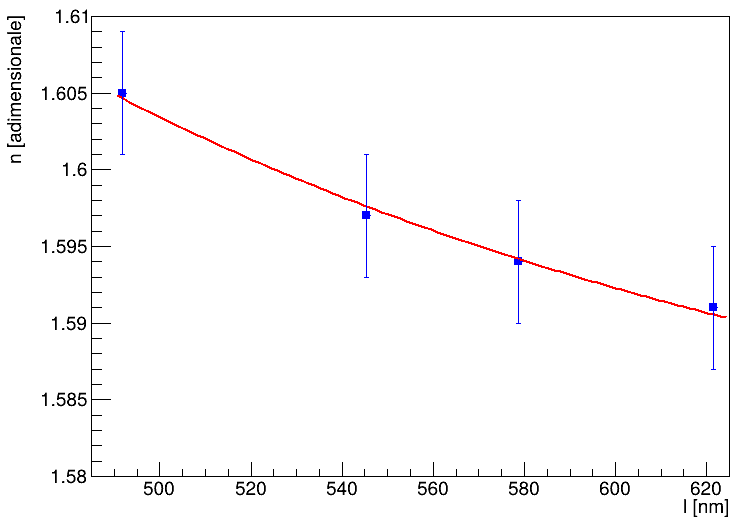
\includegraphics[width=0.7\linewidth]{Immagini/andamento n.png}
    \caption{grafico di $n(\lambda)$}
    \label{fig:andamento n}
\end{figure}

Sui dati rappresentati nel grafico in figura \ref{fig:andamento n} è stata quindi effettuata una regressione tramite la legge di Cauchy per l'indice di rifrazione
\begin{equation}
    \label{legge di Cauchy per n}
    n(\lambda)=A+\frac{B}{\lambda^2},\quad A,B\in\mathbb{R}.
\end{equation}
Il modello proposto per la regressione si adatta all'intero range di dati ($\chi^2=0.62$ e $DOF=2$), il quale pertanto risulta appropriato per descrivere l'andamento dei dati. Dunque, la regressione restituisce un valore di $A=1.57\pm0.01$, il quale fornisce una stima dell'indice di rifrazione $n$ del prisma. Questo valore è compatibile con i valori noti di $n$ del vetro crown, i quali si aggirano intorno al valore di $n\approx1.52$.

\end{document}